
\begin{frame}
  \frametitle{Software demonstration}
  \rfn
  \framesubtitle{Evaluating the REGAE solenoid\footcite{Disser}}
  \begin{figure}
    \hspace{-0.5cm}\subfloat[Testing the model]{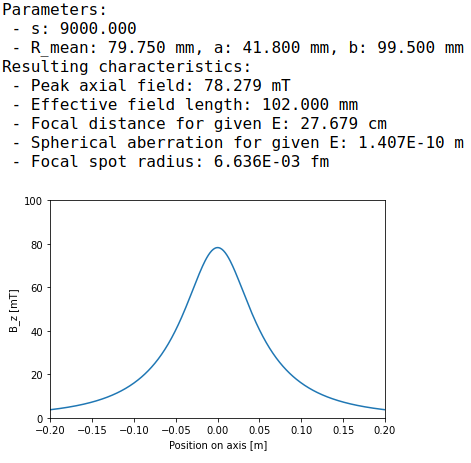
\includegraphics[width=0.5\textwidth]{calc_REGAE}}
    \hspace{0.5cm}\subfloat[Attempting to optimize within 10\% margin]{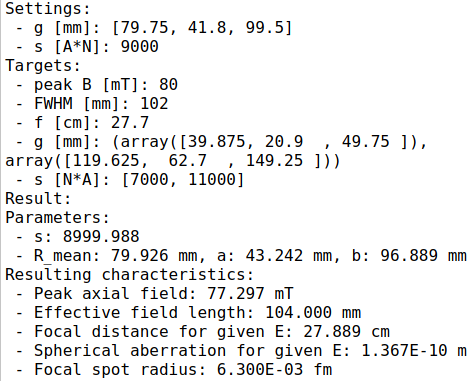
\includegraphics[width=0.5\textwidth]{opt_REGAE}}

  \end{figure}
\end{frame}

\begin{frame}
  \rfn
  \frametitle{Software demonstration}
  Results depend on initial conditions:
  \begin{figure}
    \hspace{-0.5cm}\subfloat[Optimizing for initial specifications]{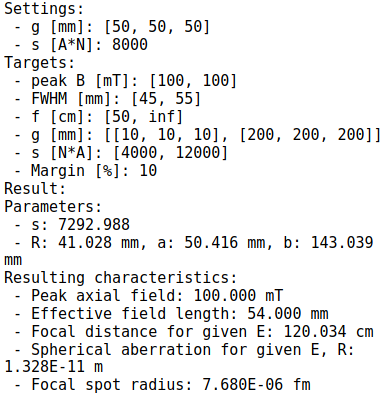
\includegraphics[width=0.5\textwidth]{opt_ok}}
    \hspace{0.5cm}\subfloat[An approach from different start values]{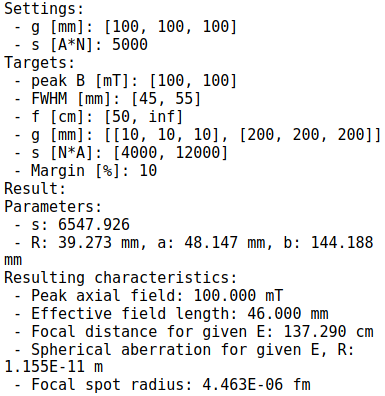
\includegraphics[width=0.5\textwidth]{opt_ok2}}

  \end{figure}
\end{frame}

\begin{frame}
  \rfn
  \frametitle{Software demonstration - observations}
  \begin{columns}
    \begin{column}{0.5\textwidth}
    \begin{figure}
      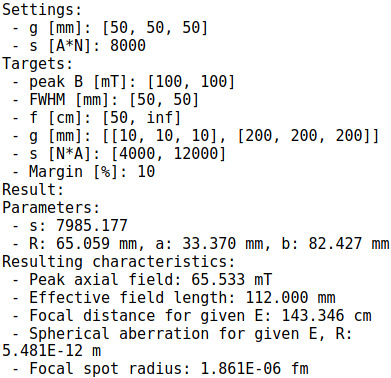
\includegraphics[width=\textwidth]{opt_overcon}
      \caption{Example of overconstraining}
    \end{figure}
    \end{column}
    \begin{column}{0.5\textwidth}
      \begin{itemize}
        \item Overconstraining throws the algorithm off
        \vspace{0.4cm}
        \item Multiple configurations in $(s, r, a, b)$ correspond to same minima\\
          \rarrow convergence depends on initial guess and search region
        \vspace{0.4cm}
        \item Parameters, constraints seem to be weighted differently - the optimization space is not normalized
        \vspace{0.4cm}
        \item Lower $c_s$ does not always yield better spot size
      \end{itemize}
    \end{column}
  \end{columns}
\end{frame}

\begin{frame}
  \frametitle{Interior point Algorithm results}
  \rfn
  \framesubtitle{Retrieved parameters}
    \begin{figure}
    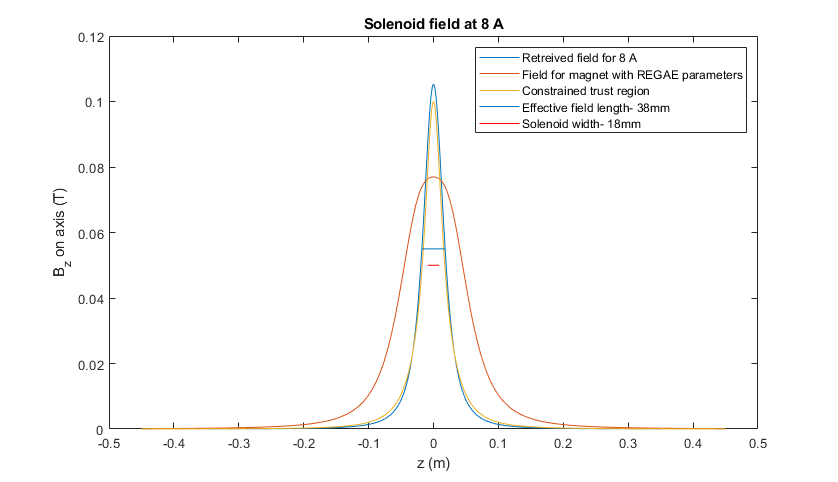
\includegraphics[width=.8\textwidth]{retreivedBz.png}
  \end{figure}
    \begin{tiny}
    \begin{table}[t]
    \centering
    \begin{tabular}{    m{1.4cm}|| m{0.9cm}| m{0.9cm} | m{1.2cm}| m{1.1cm}| m{1.5cm}| m{1.5cm}}
    & \underline{Height $a$ mm} & \underline{Width $b$ mm}& \underline{Max field $ B_z$ mT}& \underline{F. length $f$ cm}& \underline{Spherical ab. $C_s$ }& \underline{RMS emi. $\epsilon_{n.rms}$ } \\
    Opt. parameters    &17.6 & 17.6 &105& 50   &$1.7e-9 m$   &$3.4e-10 m$\\
    REGAE\footcite{Disser} & 99.5 & 41.8&79  & 30.5&$6.3e-11 m$ &$7.9e-11 m$\\
  \end{tabular}
  \end{table}
    \end{tiny}
\end{frame}

\begin{frame}
  \frametitle{Interior point Algorithm results}
  \rfn
  \framesubtitle{$F_3$ Integral}
  \begin{figure}
    \centering
    \subfloat[]{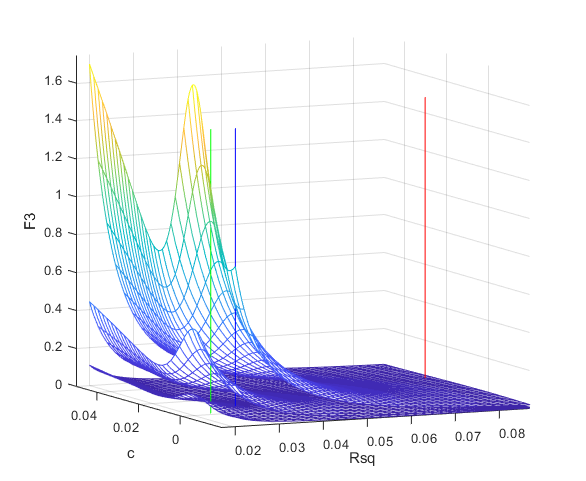
\includegraphics[width = 0.5\textwidth]     {F3.png}}
    \subfloat[]{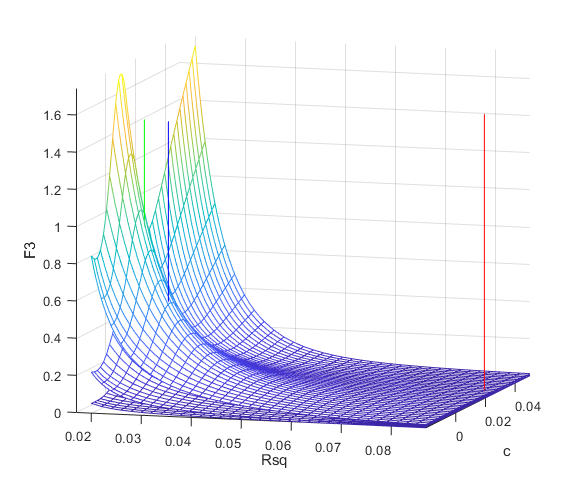
\includegraphics[width = 0.5\textwidth]{F33.png}}
    \label{some example}
    \caption{$F_3$ integral}
  \end{figure}
\end{frame}
